\chapter{Introduction}
\label{chap:intro}

\section{Motivation}
\label{sect:motivation}
LiDAR senors provide critical depth information for autonomous driving and robotics. The LiDAR intensity maps are often spares and incomplete. Using depht maps as an addtional input is a way to impove the richness and accuracy ot the LiDAR predection. The Pix2Pix network for image-to-image translation offers a promising approch for integrating these modalities. 
\section{Contribution}
This project explores the use of the Pix2Pix network to predict LiDAR intensity maps by leveraging RGB images and depth maps as additional inputs.
\section{Related Work}
DeptAnything Models: \newline DepthAnything represents a significant advancement in monocular depth estimation by leveraging both labeled and unlabeled data at a large scale. Trained on 1.5 million labeled images and over 62 million unlabeled images, DepthAnything achieves state-of-the-art performance in depth estimation tasks. The model excels in both zero-shot relative and metric depth estimation, outperforming previous models such as MiDaS v3.1 and ZoeDepth. 
\newline
version 2
\newline
3D Reconstruction Techniques: 3D reconstruction is a broad field focused on creating three-dimensional models from two-dimensional images or depth data. Techniques in 3D reconstruction include methods like structure-from-motion (SfM), multi-view stereo (MVS), and volumetric approaches. These techniques aim to generate accurate 3D representations of scenes or objects from multiple views or depth sensors.

\chapter{Preparations}
used google colab, pix2pix network getting the right input, pix2pix problems



\begin{figure}[!ht]
	\centering
	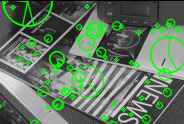
\includegraphics[width=0.9\linewidth]{image.jpg}
	\caption{caption.}
	\label{img:example}
\end{figure}
\chapter{Predicting LIDAR Intensity from RGB and Depth Images}
\section{Setup}
The used the bp net it is for depth completion and depth prediction
pix2pix model with modified data loader to get 4 dim. input rgb plus depth
used base model for depthanything
The setup for this project involved configuring a series of models and datasets to predict LIDAR intensity from RGB and depth images. The key components and their roles are outlined below:

\subsection{Bilateral Propagation Network (BP Net)}
\begin{itemize}
	\item \textbf{Purpose:} Used for depth completion to improve depth maps from incomplete or noisy data.
	\item \textbf{Dataset:} Trained and evaluated on the KITTI dataset to refine depth estimations.
\end{itemize}

\subsection{Depth Anything Models}
\begin{itemize}
	\item \textbf{Depth Anything v1:} Provided initial depth estimations using large-scale unlabeled data for zero-shot learning.
	\item \textbf{Depth Anything v2:} Enhanced depth prediction capabilities, incorporating improvements over v1 for better depth map accuracy.
\end{itemize}

\subsection{Metric Depth Estimation}
\begin{itemize}
	\item \textbf{Purpose:} Supplemented depth maps with precise metric depth measurements to enhance model performance.
\end{itemize}

\subsection{Dataset}
\begin{itemize}
	\item \textbf{Source:} KITTI dataset, containing RGB images and corresponding depth maps.
	\item \textbf{Preparation:} Combined RGB images with depth maps generated by BP Net and Depth Anything models.
\end{itemize}

\subsection{pix2pix Network}
\begin{itemize}
	\item \textbf{Purpose:} To predict LIDAR intensity from RGB and depth images.
	\item \textbf{Training Data:} RGB and depth pairs from the KITTI dataset.
\end{itemize}

\section{Implementation}
The implementation details focus on how the above components were practically applied and integrated:

\subsection{Data Preprocessing}
\begin{itemize}
	\item \textbf{Depth Map Generation:} Utilized BP Net and Depth Anything models to generate depth maps from the KITTI dataset. Depth maps were processed to ensure consistency and accuracy before use.
	\item \textbf{Dataset Preparation:} RGB images were paired with the generated depth maps to create a comprehensive training dataset for the pix2pix model.
\end{itemize}

\subsection{Model Training}
\begin{itemize}
	\item \textbf{pix2pix Configuration:} Adapted the pix2pix architecture to accept RGB images and depth maps as inputs. The network was trained to predict LIDAR intensity values based on these inputs.
	\item \textbf{Training Process:} Configured training parameters such as learning rate, batch size, and number of epochs. The model was trained using the prepared dataset to optimize performance in predicting LIDAR intensity.
\end{itemize}
\section{Results}
test run rgb only. depht from depthanything the depth from depthanything v2 and metriv form depthanything v2 6 runs with different solution
\chapter{Conclusion}
\section{Appendix}
ere is a citation for the Depth Anything paper \cite{depthanything}, its version 2 \cite{depth_anything_v2}, and for the paper by Saxena et al. \cite{saxena2008depth}

\section{References}
bp net work
pix2pix
depth anything v1 2
paper for them 
some for lidar intensity
